\begin{name}
	{\tenchude}{\tendethi}{LỚP TOÁN THẦY PHÁT}{\thoigian}
\end{name}
\setcounter{ex}{0}\setcounter{bt}{0}
\Opensolutionfile{ans}[ans/ans-2-TT-22-SGD-BaRiaVungTau-23]
\begin{ex}%[Đề TT, Sở Bà Rịa - Vũng Tàu, 2022 - 2023]%[Phạm Tiến Long , 12-EX-6-2023]%[2D2B6-1]
	Tập nghiệm $S$ của bất phương trình $\log _{\tfrac{1}{2}}(x+1)<\log _{\tfrac{1}{2}}(2 x-1)$ là
	\choice
	{$S=(2 ;+\infty)$}
	{$S=(-\infty ; 2)$}
	{\True $S=\left(\dfrac{1}{2}; 2\right)$}
	{$S=(-1 ; 2)$}
\loigiai{
Ta có $\log _{\tfrac{1}{2}}(x+1)<\log _{\tfrac{1}{2}}(2 x-1)\Leftrightarrow \heva{&x+1>0\\&2x-1>0\\&x+1>2x-1}\Leftrightarrow \heva{&x>-1\\&x>\dfrac{1}{2}\\&x<2}\Leftrightarrow \dfrac{1}{2}<x<2$.\\
Vậy tập nghiệm của bất phương trình đã cho là $S=\left(\dfrac{1}{2};2\right)$.
}	
\end{ex}

\begin{ex}%[Đề TT, Sở Bà Rịa - Vũng Tàu, 2022 - 2023]%[Phạm Tiến Long , 12-EX-6-2023]%[2D3B2-2]
	Cho $\displaystyle\int\limits_{0}^{4} f(x) \mathrm{\,d}x=16$, khi đó $\displaystyle\int\limits_{0}^{2} f(2x) \mathrm{\,d}x$ bằng
	\choice
	{$32$}
	{\True $8$}
	{$16$}
	{$4$}
	\loigiai{
		Đặt $t=2x\Rightarrow \mathrm{\,d}t=2\mathrm{\,d}x$. Đổi cận $x=0\Rightarrow t=0$, $x=2\Rightarrow t=4$. Khi đó
		$$\displaystyle\int\limits_{0}^{2} f(2x) \mathrm{\,d}x= \displaystyle\int\limits_{0}^{4} f(t) \dfrac{1}{2}\mathrm{\,d}t=\dfrac{1}{2} \displaystyle\int\limits_{0}^{4} f(t) \mathrm{\,d}t=\dfrac{1}{2} \cdot 16=8.$$
	}
\end{ex}

\begin{ex}%[Đề TT, Sở Bà Rịa - Vũng Tàu, 2022 - 2023]%[Phạm Tiến Long , 12-EX-6-2023]%[2D1Y5-1]
\immini
{
Đồ thị của hàm số nào dưới đây có dạng như đường cong trong hình bên?
\choice
{$y=x^3-3x$}
{$y=x^2-3x$}
{\True $y=x^4-3x^2$}
{$y=\dfrac{x}{x-3}$}}
{
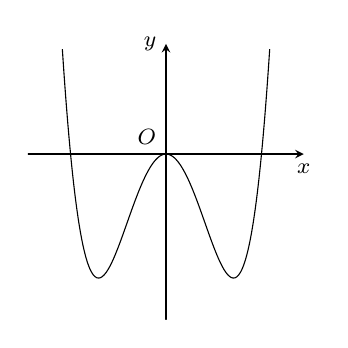
\begin{tikzpicture}[scale=0.7, font=\footnotesize, line join=round, line cap=round, >=stealth]
 \def\xmin{-2.5} \def\xmax{2.5}
 \def\ymin{-3} \def\ymax{2} 
 \draw[->] (\xmin,0)--(\xmax,0) node [below]{$x$};
 \draw[->] (0,\ymin)--(0,\ymax) node [left]{$y$};
 \clip (\xmin+0.1,\ymin+0.1) rectangle (\xmax-0.1,\ymax-0.1);
 \draw[smooth,samples=300] plot(\x,{(\x)^4-3*(\x)^2});
\fill (0,0)circle (1pt)node[above left]{$O$};
\end{tikzpicture}
}
\loigiai{
Dựa vào hình vẽ ta thấy đây là đồ thị của hàm số dạng $y=ax^4+bx^2+c$ với $a>0$. \\
Chỉ có phương án $y=x^4-3x^2$ thỏa mãn.
}
\end{ex}

\begin{ex}%[Đề TT, Sở Bà Rịa - Vũng Tàu, 2022 - 2023]%[Phạm Tiến Long , 12-EX-6-2023]%[2D2B5-1]
	Nghiệm của phương trình $2^{x+1}=5$ là
	\choice
	{$x=\log _{2}5$}
	{$x=1-\log _{2}5$}
	{\True $x=-1+\log _{2}5$}
	{$x=-1+\log _{5}2$}
	\loigiai{
		Ta có $2^{x+1}=5 \Leftrightarrow x+1=\log _{2}5 \Leftrightarrow x=-1+\log _{2}5$.
	}
\end{ex}

\begin{ex}%[Đề TT, Sở Bà Rịa - Vũng Tàu, 2022 - 2023]%[Phạm Tiến Long , 12-EX-6-2023]%[2D3Y2-1]
	Cho hàm số $f(x)$ có đạo hàm trên đoạn $[1;2]$, $f(1)=1$ và $f(2)=2$ thì $\displaystyle\int\limits_1^2 f'(x) \mathrm{\,d}x$ bằng
	\choice
	{\True $1$}
	{$-1$}
	{$3$}
	{$\dfrac{7}{2}$}
\loigiai{
Ta có $\displaystyle\int\limits_1^2 f'(x) \mathrm{\,d}x=f(2)-f(1)=1$.
}
\end{ex}

\begin{ex}%[Đề TT, Sở Bà Rịa - Vũng Tàu, 2022 - 2023]%[Phạm Tiến Long , 12-EX-6-2023]%[2D1Y2-2]
	Cho hàm số $y=f(x)$ có bảng biến thiên như sau
	\begin{center}
		
\begin{tikzpicture}
			\tkzTabInit[nocadre=false, lgt=1.2, espcl=2.5, deltacl=0.6]
			{$x$/0.6,$y'$/0.6,$y$/2}
			{$-\infty$, $0$, $2$, $+\infty$}
			\tkzTabLine {,-,0,+,0,-,}
			\tkzTabVar{+/$+\infty$, -/$1$, +/$5$, -/$-\infty$}
		\end{tikzpicture}
	\end{center}
	Điểm cực đại của hàm số là
	\choice
	{$x=5$}
	{\True $x=2$}
	{$x=0$}
	{$x=1$}
	\loigiai{
		Dựa vào bảng biến thiên, ta thấy điểm cực đại của hàm số là $x=2$.
	}
\end{ex}

\begin{ex}%[Đề TT, Sở Bà Rịa - Vũng Tàu, 2022 - 2023]%[Phạm Tiến Long , 12-EX-6-2023]%[2D2Y3-2]
Với $a$, $b$ là các số thực dương tùy ý. Mệnh đề nào dưới đây đúng?
\choice
{\True $\ln(ab)=\ln a+\ln b$}
{$\ln(ab)=\ln a\cdot\ln b$}
{$\ln \dfrac{a}{b}=\dfrac{\ln a}{\ln b}$}
{$\ln \dfrac{a}{b}=\ln b-\ln a$}
\loigiai{
Mệnh đề đúng là $\ln(ab)=\ln a+\ln b$.
}
\end{ex}

\begin{ex}%[Đề TT, Sở Bà Rịa - Vũng Tàu, 2022 - 2023]%[Phạm Tiến Long , 12-EX-6-2023]%[2H3Y3-5]
	Cho đường thẳng $\Delta$ cắt mặt cầu $S(O;R)$. Gọi $d$ là khoảng cách từ $O$ đến $\Delta$. Khẳng định nào dưới đây đúng?
	\choice
	{\True $d<R$}
	{$d>R$}
	{$d=R$}
	{$d=0$}
	\loigiai{
		Ta có $\Delta$ cắt mặt cầu  $S(O;R)$ nên suy ra  $\mathrm{d}\left(O,\Delta\right)<R$.
	}
\end{ex}

\begin{ex}%[Đề TT, Sở Bà Rịa - Vũng Tàu, 2022 - 2023]%[Phạm Tiến Long , 12-EX-6-2023]%[2H1Y3-2]
	Cho khối lăng trụ tứ giác có đáy là hình vuông cạnh bằng $4$, chiều cao bằng $6$. Thể tích của khối lăng trụ đã cho bằng
	\choice
	{\True $96$}
	{$16$}
	{$24$}
	{$32$}
	\loigiai{
Ta có	$V=Sh=4^2 \cdot 6=96$.
	}
\end{ex}

\begin{ex}%[Đề TT, Sở Bà Rịa - Vũng Tàu, 2022 - 2023]%[Phạm Tiến Long , 12-EX-6-2023]%[2H3Y1-3]
	Trong không gian $Oxyz$, cho mặt cầu $(S)\colon(x+1)^{2}+(y+2)^{2}+z^{2}=5$. Toạ độ tâm $I$ và bán kính $R$ của $(S)$ là
	\choice
	{$I(1;2;0)$, $R=5$}
	{$I(1;2;0)$, $R=\sqrt{5}$}
	{\True $I(-1;-2;0)$, $R=\sqrt{5}$}
	{$I(-1;-2;0)$, $R=5$}
	\loigiai{
		Mặt cầu $(S)$ đã cho có tâm $I(-1;-2;0)$ và bán kính $R=\sqrt{5}$.
	}
\end{ex}

\begin{ex}%[Đề TT, Sở Bà Rịa - Vũng Tàu, 2022 - 2023]%[Phạm Tiến Long , 12-EX-6-2023]%[2D2B3-2]
	Đặt $a=\log _3 2$, khi đó $\log _{16}27$ bằng
	\choice
	{$\dfrac{3a}{4}$}
	{$\dfrac{4a}{3}$}
	{$\dfrac{4}{3a}$}
	{\True $\dfrac{3}{4a}$}
	\loigiai{
	Ta có $\log_{16}27=\log_{2^4}3^3=\dfrac{3}{4}\log_2 3=\dfrac{3}{4}\cdot \dfrac{1}{\log _3 2}=\dfrac{3}{4a}$.
}	
\end{ex}

\begin{ex}%[Đề TT, Sở Bà Rịa - Vũng Tàu, 2022 - 2023]%[Phạm Tiến Long , 12-EX-6-2023]%[2H1B3-2]
	Cho khối lăng trụ tam giác đều có tất cả các cạnh bằng $a$. Thể tích khối lăng trụ đã cho bằng
	\choice
	{$V=\dfrac{a^{3}\sqrt{3}}{6}$}
	{$V=\dfrac{a^{3}\sqrt{3}}{12}$}
	{$V=\dfrac{a^{3}\sqrt{3}}{2}$}
	{\True $V=\dfrac{a^{3}\sqrt{3}}{4}$}
	\loigiai{
		\immini{
			Khối lăng trụ tam giác đều có $h=AA'=a$ và diện tích đáy $S_{ABC}=\dfrac{a^2\sqrt{3}}{4}$.\\
			Vậy thể tích của khối lăng trụ đã cho là $V=S_{ABC}\cdot h=\dfrac{a^2\sqrt{3}}{4}\cdot a=\dfrac{a^3 \sqrt{3}}{4}$.
		}{
			\begin{tikzpicture}[scale=0.7, font=\footnotesize, line join=round, line cap=round, >=stealth]
				\def\h{1.5}
				\path
				(0,0) coordinate (A)
				(2,-1) coordinate (B)
				(3,0) coordinate (C)
				($(A)+(0,\h)$) coordinate (A')
				($(A')+(B)$) coordinate (B')
				($(A')+(C)$) coordinate (C')
				;
				\draw (B)--(B')--(A')--(A)--(B)--(C)--(C')--(B') (A')--(C');
				\draw[dashed] (A)--(C);
				\foreach \d/\g in {A/-170,B/-90,C/-20,A'/170,B'/90,C'/20}{
					\draw[fill=black](\d) circle (1pt) +(\g:.3)node{$\d$};}
		\end{tikzpicture}	}	
	}
\end{ex}

\begin{ex}%[Đề TT, Sở Bà Rịa - Vũng Tàu, 2022 - 2023]%[Phạm Tiến Long , 12-EX-6-2023]%[2H2B1-2]
	Cho hình nón có diện tích xung quanh bằng $3 \pi a^2$ và có bán kính đáy bằng $a$. Độ dài đường sinh của hình nón đã cho bằng
	\choice
	{$2a$}
	{$\dfrac{3a}{2}$}
	{$2\sqrt{2}a$}
	{\True $3a$}
	\loigiai{
Ta có $S_{\text{xq}}=\pi rl \Leftrightarrow 3 \pi a^2=\pi  a l \Rightarrow l=\dfrac{3\pi a^2}{\pi a}=3 a$.	
}
\end{ex}

\begin{ex}%[Đề TT, Sở Bà Rịa - Vũng Tàu, 2022 - 2023]%[Phạm Tiến Long , 12-EX-6-2023]%[2H3Y2-2]
	Trong không gian $Oxyz$, mặt phẳng $(P)\colon x-2z+1=0$ có một véc-tơ pháp tuyến là
	\choice
	{$\overrightarrow{n_2}=(0;1;-2)$}
	{$\overrightarrow{n_3}=(1;-2;0)$}
	{\True $\overrightarrow{n_1}=(1;0;-2)$}
	{$\overrightarrow{n_4}=(1;-2;1)$}
	\loigiai{
		Mặt phẳng $(P)$ có một véc-tơ pháp tuyến là $\overrightarrow{n}=(1;0;-2)$.
	}
\end{ex}

\begin{ex}%[Đề TT, Sở Bà Rịa - Vũng Tàu, 2022 - 2023]%[Phạm Tiến Long , 12-EX-6-2023]%[2D2Y2-1]
	Tập xác định $\mathscr{D}$ của hàm số $y=\left(x^2-x-2\right)^{-3}$ là
	\choice
	{$\mathscr{D}=\mathbb{R}$}
	{$\mathscr{D}=(0;+\infty)$}
	{\True $\mathscr{D}=\mathbb{R}\backslash\{-1;2\}$}
	{$\mathscr{D}=(-\infty;-1) \cup(2 ;+\infty)$}
\loigiai{
Hàm số đã cho xác định khi $x^2-x-2 \ne 0\Leftrightarrow \heva{&x\ne -1\\&x\ne 2.}$\\
Vậy tập xác định của hàm số đã cho là $\mathscr{D}=\mathbb{R}\backslash\{-1;2\}$.
}
\end{ex}

\begin{ex}%[Đề TT, Sở Bà Rịa - Vũng Tàu, 2022 - 2023]%[Phạm Tiến Long , 12-EX-6-2023]%[2H3B2-5]
	Trong không gian $Oxyz$, góc giữa hai mặt phẳng $(Oxz)$ và $(P)\colon x-y+1=0$ bằng
	\choice
	{$60^{\circ}$}
	{$135^{\circ}$}
	{\True $45^{\circ}$}
	{$90^{\circ}$}
	\loigiai{
		Mặt phẳng $(Oxz)$ có một véc-tơ pháp tuyến là $\overrightarrow{j}=(0;1;0)$, $(P)$ có một véc-tơ pháp tuyến là $\overrightarrow{n}=(1;-1;0)$. Khi đó
		$$\cos \left((Oxz),(P)\right)=\left|\cos \left(\overrightarrow{j}, \overrightarrow{n}\right)\right|=\dfrac{|\overrightarrow{j}\cdot \overrightarrow{n}|}{|\overrightarrow{j}|\cdot  |\overrightarrow{n}|}=\dfrac{|0\cdot 1 +1\cdot (-1) + 0 \cdot 0 |}{\sqrt{0^2+1^2+0^2}\cdot \sqrt{1^2+(-1)^2+0^2}}=\dfrac{\sqrt{2}}{2}.$$
		Vậy $\left((Oxz),(P)\right)=45^{\circ}$.
	}
\end{ex}

\begin{ex}%[Đề TT, Sở Bà Rịa - Vũng Tàu, 2022 - 2023]%[Phạm Tiến Long , 12-EX-6-2023]%[2D2Y4-2]
	Đạo hàm của hàm số $y=5^x$ là
	\choice
	{$y'=x\cdot 5^{x-1}$}
	{\True $y'=5^x \cdot \ln 5$}
	{$y'=5^x$}
	{$y'=\dfrac{5^x}{\ln 5}$}
	\loigiai{
Ta có $y'=5^x \cdot \ln 5$.	
}
\end{ex}

\begin{ex}%[Đề TT, Sở Bà Rịa - Vũng Tàu, 2022 - 2023]%[Phạm Tiến Long , 12-EX-6-2023]%[2D3B2-1]
	Nếu $\displaystyle\int\limits_{0}^{\frac{\pi}{2}} f(x) \mathrm{\,d}x=5$ thì $\displaystyle\int\limits_{0}^{\frac{\pi}{2}} [f(x)+2 \sin x] \mathrm{\,d}x$ bằng
	\choice
	{\True $7$}
	{$5+\dfrac{\pi}{2}$}
	{$3$}
	{$5+\pi$}
	\loigiai{
		Ta có $\displaystyle\int\limits_{0}^{\frac{\pi}{2}} [f(x)+2 \sin x] \mathrm{\,d}x = \displaystyle\int\limits_{0}^{\frac{\pi}{2}} f(x) \mathrm{\,d}x + 2 \displaystyle\int\limits_{0}^{\frac{\pi}{2}} \sin x \mathrm{\,d}x = 5+ 2 (-\cos x)\Big|_0^{\frac{\pi}{2}}= 5+2(0+1)=7$.
	}
\end{ex}

\begin{ex}%[Đề TT, Sở Bà Rịa - Vũng Tàu, 2022 - 2023]%[Phạm Tiến Long , 12-EX-6-2023]%[2D1B4-1]
	Đồ thị của hàm số nào dưới đây có tiệm cận đứng?
	\choice
	{$y=\dfrac{x^2}{x^2+1}$}
	{$y=\dfrac{x^2-3x+2}{x-1}$}
	{$y=\sqrt{x^2-1}$}
	{\True $y=\dfrac{x}{x+1}$}
\loigiai{
Xét hàm số $y=\dfrac{x}{x+1}$ có tập xác định là $\mathscr{D}=\mathbb{R}\backslash\{-1\}$.\\
Ta có $\lim\limits_{x\to -1^-}y=+\infty$ và $\lim\limits_{x\to -1^+}y=-\infty$.\\
Nên đồ thị hàm số $y=\dfrac{x}{x+1}$ có tiệm cận đứng là $x=-1$.
}
\end{ex}

\begin{ex}%[Đề TT, Sở Bà Rịa - Vũng Tàu, 2022 - 2023]%[Phạm Tiến Long , 12-EX-6-2023]%[2D1B3-1]
	Giá trị nhỏ nhất của hàm số $y=x^4-12x^2+10$ trên $[0;6]$ đạt tại điểm
	\choice
	{\True $x=\sqrt{6}$}
	{$x=0$}
	{$x=-26$}
	{$x=6$}
	\loigiai{
		Tập xác định của hàm số là $\mathbb{R}$, $y'=4x^3-24x=4x(x^2-6)$ và $y'=0\Leftrightarrow 4x(x^2-6)=0 \Leftrightarrow \hoac{& x=0\\& x=\pm \sqrt{6}.}$\\
		Xét trên $[0;6]$, ta có $y(0)=10$, $y(\sqrt{6})=-26$, $y(6)=874$.\\
		Vậy hàm số đã cho có giá trị nhỏ nhất là $-26$, đạt tại $x=\sqrt{6}$.
	}
\end{ex}

\begin{ex}%[Đề TT, Sở Bà Rịa - Vũng Tàu, 2022 - 2023]%[Phạm Tiến Long , 12-EX-6-2023]%[1D2Y2-1]
	Từ các chữ số $1$, $2$, $3$, $4$, $5$, $6$, $7$ lập được bao nhiêu số tự nhiên gồm hai chữ số khác nhau?
	\choice
	{$\mathrm{C}_7^2$}
	{$2^7$}
	{$7^2$}
	{\True $\mathrm{A}_7^2$}
	\loigiai{
Số các số tự nhiên gồm hai chữ số khác nhau được lập từ các chữ số đã cho là $\mathrm{A}_7^2$ (số).	
}
\end{ex}

\begin{ex}%[Đề TT, Sở Bà Rịa - Vũng Tàu, 2022 - 2023]%[Phạm Tiến Long , 12-EX-6-2023]%[1D3Y3-3]
	Cho cấp số cộng $(u_n)$ với $u_1=2$ và công sai $d=3$. Giá trị của $u_3$ bằng
	\choice
	{$18$}
	{\True $8$}
	{$6$}
	{$11$}
	\loigiai{
		Ta có $u_3=u_1+2d=2+2\cdot 3=8$.
	}
\end{ex}

\begin{ex}%[Đề TT, Sở Bà Rịa - Vũng Tàu, 2022 - 2023]%[Phạm Tiến Long , 12-EX-6-2023]%[2D1Y5-4]
	Cho hàm số $y=x^3+5 x$ có đồ thị $(C)$. Số giao điểm của $(C)$ với trục hoành là
	\choice
	{$3$}
	{$1$}
	{$0$}
	{$0$}
\loigiai{
	Phương trình hoành độ giao điểm của $(C)$ với trục hoành là $x^3+5 x=0 \Leftrightarrow x\left(x^2+5\right)=0 \Leftrightarrow x=0$.\\
Vậy có $1$ giao điểm của $(C)$ với trục hoành.
}
\end{ex}

\begin{ex}%[Đề TT, Sở Bà Rịa - Vũng Tàu, 2022 - 2023]%[Phạm Tiến Long , 12-EX-6-2023]%[2D1Y1-1]
	Cho hàm số $y=f(x)$ có đạo hàm $f'(x)=3x^2, ~\forall x \in \mathbb{R}$. Khẳng định nào dưới đây đúng?
	\choice
	{Hàm số nghịch biến trên $(-\infty;0)$}
	{Hàm số nghịch biến trên $(0;+\infty)$}
	{Hàm số nghịch biến trên $(-\infty;+\infty)$}
	{\True Hàm số đồng biến trên $(-\infty;+\infty)$}
	\loigiai{
		Ta có $f'(x)\ge 0, ~\forall x \in \mathbb{R}$ nên hàm số đã cho đồng biến trên $(-\infty;+\infty)$.
	}
\end{ex}

\begin{ex}%[Đề TT, Sở Bà Rịa - Vũng Tàu, 2022 - 2023]%[Phạm Tiến Long , 12-EX-6-2023]%[2D1Y1-2]
\immini
{
Cho hàm số $y=f(x)$ có đồ thị như hình vẽ bên. Hàm số đã cho đồng biến trên khoảng nào dưới đây?
\choice
{$(0;1)$}
{$(-\infty;1)$}
{$(-1;1)$}
{\True $(-1;0)$}}
{
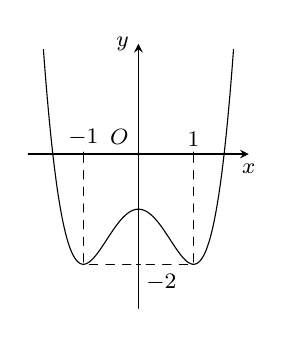
\begin{tikzpicture}[scale=0.7, font=\footnotesize, line join=round, line cap=round, >=stealth]
 \def\xmin{-2} \def\xmax{2}
 \def\ymin{-2.8} \def\ymax{2} 
 \draw[->] (\xmin,0)--(\xmax,0) node [below]{$x$};
 \draw[->] (0,\ymin)--(0,\ymax) node [left]{$y$};
 \clip (\xmin+0.1,\ymin+0.1) rectangle (\xmax-0.1,\ymax-0.1);
 \draw[smooth,samples=300] plot(\x,{(\x)^4-2*(\x)^2-1});
\fill (0,0)circle (1pt)node[above left]{$O$};
\foreach \x/\g in {-1/above,1/above}  \draw[thin] (\x,1pt)--(\x,-1pt) node[\g]{$\x$};
\foreach \y/\g in {-2/below right} \draw[thin] (1pt,\y)--(-1pt,\y) node[\g]{$\y$}; 
\draw[dashed] (-1,0)--(-1,-2)--(0,-2) (1,0)--(1,-2)--(0,-2);
\end{tikzpicture}
}
\loigiai{
Dựa vào hình vẽ ta có hàm số đã cho đồng biến trên khoảng $(-1;0)$ và $(1;+\infty)$.
}
\end{ex}

\begin{ex}%[Đề TT, Sở Bà Rịa - Vũng Tàu, 2022 - 2023]%[Phạm Tiến Long , 12-EX-6-2023]%[2D1Y2-2]
	\immini{
		Cho hàm số bậc ba $y=f(x)$ có đồ thị là đường cong như hình bên. Giá trị cực tiểu của hàm số đã cho là
		\choice
		{\True $-1$}
		{$1$}
		{$2$}
		{$3$}
	}{
		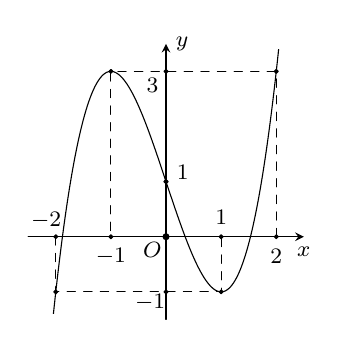
\begin{tikzpicture}[scale=0.7, font=\footnotesize, line join=round, line cap=round, >=stealth]
			\def\xt{-2.5} \def\xp{2.5} \def\yd{-1.5} \def\yt{3.5}
			\draw[->] (\xt,0)--(\xp,0) node [below]{$x$};
			\draw[->] (0,\yd)--(0,\yt) node [right]{$y$};
			\draw[fill=black](0,0) circle (1.5pt) +(-135:0.35)node{$O$};
			\clip (\xt+0.1,\yd+0.1) rectangle (\xp-0.1,\yt-0.1);
			\draw[smooth,samples=300,domain=\xt:\xp] plot(\x,{(\x)^3-3*(\x)+1});
			\foreach \i/\g in {-2/120,-1/-90,1/90,2/-90}{
				\draw[fill=black](\i,0) circle (1pt) +(\g:0.35)node{$\i$};}
			\foreach \j/\g in {-1/-145,1/30,3/-135}{
				\draw[fill=black](0,\j) circle (1pt) +(\g:0.35)node{$\j$};}
			\foreach \x/\y in {-2/-1,-1/3,1/-1,2/3,0/1}{
				\draw[fill=black](\x,\y) circle (1pt);}
			\draw[dashed] (2,0)|-(0,3)-|(-1,0); \draw[dashed] (-2,0)|-(0,-1)-|(1,0);
	\end{tikzpicture}}
	\loigiai{
		Dựa vào đồ thị hàm số đã cho, ta thấy giá trị cực tiểu của hàm số đã cho là $y_{\text{CT}}=-1$.
	}
\end{ex}

\begin{ex}%[Đề TT, Sở Bà Rịa - Vũng Tàu, 2022 - 2023]%[Phạm Tiến Long , 12-EX-6-2023]%[2D3Y1-1]
	Họ nguyên hàm của hàm số $f(x)=\mathrm{e}^x+x$ là
	\choice
	{ $\mathrm{e}^x+x^2+C$}
	{\True $\mathrm{e}^x+\dfrac{1}{2}x^2+C$}
	{$\dfrac{1}{x+1}\mathrm{e}^x+\dfrac{1}{2}x^2+C$}
	{$\mathrm{e}^x+1+C$}
	\loigiai{
Ta có 
$\displaystyle\int \left(\mathrm{e}^x+x\right)\mathrm{\,d}x=\mathrm{e}^x+\dfrac{1}{2}x^2+C$.	
}
\end{ex}

\begin{ex}%[Đề TT, Sở Bà Rịa - Vũng Tàu, 2022 - 2023]%[Phạm Tiến Long , 12-EX-6-2023]%[2H1Y3-2]
	Cho khối chóp có đáy là hình vuông cạnh $a$ và chiều cao bằng $2a$. Thể tích của khối chóp đã cho bằng
	\choice
	{$4a^3$}
	{\True $\dfrac{2}{3}a^3$}
	{$2a^3$}
	{$\dfrac{4}{3}a^3$}
	\loigiai{
		Diện tích đáy hình vuông là $B=a^2$.\\
		Vậy thể tích của khối chóp đã cho là $V=\dfrac{1}{3} B h=\dfrac{1}{3}\cdot a^2\cdot 2a=\dfrac{2}{3}a^3$.
	}
\end{ex}

\begin{ex}%[Đề TT, Sở Bà Rịa - Vũng Tàu, 2022 - 2023]%[Phạm Tiến Long , 12-EX-6-2023]%[2D3B2-3]
	Biết $\displaystyle\int\limits_0^{\tfrac{\pi}{4}}x \cos 2 x \mathrm{\,d}x=a+b \pi$, với $a$, $b$ là các số hữu tỷ. Giá trị $S=a+2b$ bằng
	\choice
	{\True $0$}
	{$1$}
	{$\dfrac{1}{2}$}
	{$\dfrac{3}{8}$}
	\loigiai{
Đặt $\heva{&u=x\\&\mathrm{d}v=\cos 2x \mathrm{d}x}\Rightarrow \heva{&\mathrm{d}u=\mathrm{d}x\\&v=\dfrac{1}{2}\sin 2x.}$\\
Ta có
\begin{eqnarray*}
 \displaystyle\int\limits_0^{\tfrac{\pi}{4}}x \cos 2 x \mathrm{\,d}x &=&  \dfrac{1}{2}x\sin 2x \bigg|_0^{\tfrac{\pi}{4}}- \displaystyle\int\limits_0^{\tfrac{\pi}{4}} \dfrac{1}{2}\sin 2x \mathrm{\,d}x\\
  &= & \dfrac{\pi}{8}+\dfrac{1}{4}\cos 2x\bigg|_0^{\tfrac{\pi}{4}}\\
  &= &  \dfrac{\pi}{8}-\dfrac{1}{4}.
 \end{eqnarray*}
Suy ra $a=-\dfrac{1}{4}$, $b=\dfrac{1}{8}$.\\
Vậy $S=a+2b=0$.
}
\end{ex}


\begin{ex}%[Đề TT, Sở Bà Rịa - Vũng Tàu, 2022 - 2023]%[Phạm Tiến Long , 12-EX-6-2023]%[2D3B3-3]
	Thể tích khối tròn xoay thu được khi quay hình phẳng giới hạn bởi hai đường $y=x^2-x$ và $y=0$ quanh trục $Ox$ bằng
	\choice
	{$\dfrac{\pi}{3}$}
	{$\dfrac{\pi}{15}$}
	{\True $\dfrac{\pi}{30}$}
	{$\dfrac{\pi}{5}$}
	\loigiai{
		Phương trình hoành độ giao điểm của hai đồ thị hàm số đã cho 
		$x^2-x=0 \Leftrightarrow \hoac{& x=0\\& x=1.}$\\
		Vậy thể tích khối tròn xoay cần tìm là $V=\pi \displaystyle\int\limits_{0}^{1} (x^2-x)^2 \mathrm{\,d}x=\dfrac{\pi}{30}$.
	}
\end{ex}

\begin{ex}%[Đề TT, Sở Bà Rịa - Vũng Tàu, 2022 - 2023]%[Phạm Tiến Long , 12-EX-6-2023]%[1H3B4-3]
	\immini{
		Cho lăng trụ tam giác đều $ABC.A'B'C'$ có tất cả các cạnh bằng nhau (tham khảo hình bên). 
		Cô-sin của góc tạo bởi hai mặt phẳng $\left(A'BC\right)$ và $(ABC)$ bằng
		\choice
		{$\dfrac{2\sqrt{3}}{3}$}
		{\True $\dfrac{\sqrt{21}}{7}$}
		{$\dfrac{2\sqrt{7}}{7}$}
		{$\dfrac{\sqrt{21}}{3}$}
	}{
		\begin{tikzpicture}[scale=1, font=\footnotesize, line join=round, line cap=round, >=stealth]
			\path
			(0,3) coordinate (A')
			(1.7,2) coordinate (B')
			(3,3) coordinate (C')
			(0,0) coordinate (A)
			($(A)+(B')-(A')$) coordinate (B)
			($(B)+(C')-(B')$) coordinate (C)
			;
			\draw (A')--(B')--(C')--(C) (A)--(A')--(C') (A)--(B)--(C) (B')--(B) (A')--(B);
			\draw[dashed] (A)--(C) (A')--(C);
			\foreach \x/\g in {A'/180,B'/90,C'/0,A/180,B/270,C/0} \fill[black] (\x) circle (1pt)+(\g:0.3) node{$\x$};
		\end{tikzpicture}
	}
	\loigiai{
		\immini{
			Đặt $AA'=a$.\\
			Kẻ $AM \perp (BC)$ tại $M$.\\
			Ta có $\heva{&BC\perp AM\\&BC\perp AA'}\Rightarrow BC\perp \left(AA'M\right).$\\
			Suy ra góc giữa hai mặt phẳng $\left(A'BC\right)$ và $(ABC)$ bằng góc $\widehat{AMA'}$.\\
			Trong tam giác $AMA'$ vuông tại $A$ ta có
			$$A'M=\sqrt{AA'^2+AM^2}=\sqrt{a^2+\left(\dfrac{a\sqrt{3}}{2}\right)^2}=\dfrac{a\sqrt{7}}{2}.$$
			Suy ra $\cos \widehat{AMA'}=\dfrac{AM}{A'M}=\dfrac{a\sqrt{3}}{2}:\dfrac{a\sqrt{7}}{2}=\dfrac{\sqrt{21}}{7}$.\\
			Vậy cô-sin của góc tạo bởi hai mặt phẳng $\left(A'BC\right)$ và $(ABC)$ bằng $\dfrac{\sqrt{21}}{7}$.
		}{
			\begin{tikzpicture}[scale=1, font=\footnotesize, line join=round, line cap=round, >=stealth]
				\path
				(0,3) coordinate (A')
				(1.7,2) coordinate (B')
				(3,3) coordinate (C')
				(0,0) coordinate (A)
				($(A)+(B')-(A')$) coordinate (B)
				($(B)+(C')-(B')$) coordinate (C)	
				($(B)!1/2!(C)$) coordinate (M)
				;
				\draw (A')--(B')--(C')--(C) (A)--(A')--(C') (A)--(B)--(C) (B')--(B) (A')--(B);
				\draw[dashed] (A)--(C) (A')--(C) (A')--(M)--(A);
				\foreach \x/\g in {A'/180,B'/90,C'/0,A/180,B/270,C/0,M/270} \fill[black] (\x) circle (1pt)+(\g:0.3) node{$\x$};
		\end{tikzpicture}	}
	}
\end{ex}

\begin{ex}%[Đề TT, Sở Bà Rịa - Vũng Tàu, 2022 - 2023]%[Phạm Tiến Long , 12-EX-6-2023]%[2D1B2-1]
	Cho hàm số $y=f(x)$ có đạo hàm $f'(x)=x^2(x-1)(x+2)$ với mọi $x \in \mathbb{R}$. Số điểm cực tiểu của hàm số đã cho là
	\choice
	{$0$}
	{$3$}
	{\True $1$}
	{$2$}
	\loigiai{
		Ta có $f'(x)=0 \Leftrightarrow x^2(x-1)(x+2)=0 \Leftrightarrow \hoac{& x=0\\& x=1\\& x=-2.}$\\
		Bảng xét dấu của $f'(x)$ như sau
		\begin{center}
			
\begin{tikzpicture}
				\tkzTabInit[nocadre=false, lgt=1.2, espcl=2.5, deltacl=0.6]
				{$x$/0.6,$f'(x)$/0.6}
				{$-\infty$, $-2$, $0$ , $1$, $+\infty$}
				\tkzTabLine {,+,0,-,0,-,0,+,}
			\end{tikzpicture}
		\end{center}
		Vậy hàm số đã cho có $1$ điểm cực tiểu là $x_{\text{CT}}=1$.
	}
\end{ex}

\begin{ex}%[Đề TT, Sở Bà Rịa - Vũng Tàu, 2022 - 2023]%[Phạm Tiến Long , 12-EX-6-2023]%[2D1Y5-3]
\immini{
	Cho hàm số bậc ba $y=f(x)$ có đồ thị là đường cong như hình bên. Có bao nhiêu giá trị nguyên của tham số $m$ để phương trình $f(x)=m$ có ba nghiệm thực phân biệt?
	\choice
	{$4$}
	{$5$}
	{$2$}
	{\True $3$}
}{
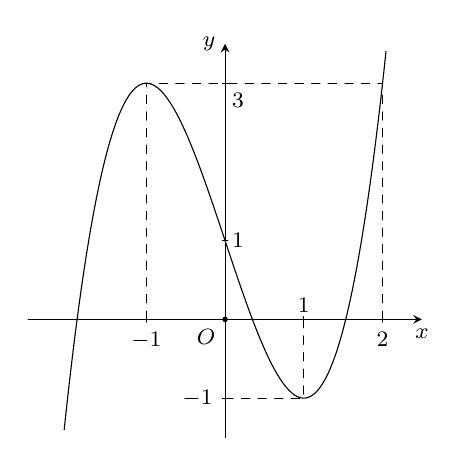
\begin{tikzpicture}[scale=1, font=\footnotesize, line join=round, line cap=round, >=stealth]
  \def\xmin{-2.5} \def\xmax{2.5}
 \def\ymin{-1.5} \def\ymax{3.5} 
 \draw[->] (\xmin,0)--(\xmax,0) node [below]{$x$};
 \draw[->] (0,\ymin)--(0,\ymax) node [left]{$y$};
 \clip (\xmin+0.1,\ymin+0.1) rectangle (\xmax-0.1,\ymax-0.1);
 \draw[smooth,samples=300] plot(\x,{(\x)^3-3*(\x)+1});
 \fill (0,0)circle (1pt)node[below left]{$O$};
 \foreach \x/\g in {-1/below,1/above,2/below}  \draw[thin] (\x,1pt)--(\x,-1pt) node[\g]{$\x$};
 \foreach \y/\g in {-1/left,1/right,3/below right} \draw[thin] (1pt,\y)--(-1pt,\y) node[\g]{$\y$};
 \draw[dashed] (-1,0)--(-1,3)--(0,3) (1,0)--(1,-1)--(0,-1) (2,0)--(2,3)--(0,3);
\end{tikzpicture}
}
\loigiai{
Dựa vào hình vẽ ta thấy phương trình $f(x)=m$ có nghiệm thực phân biệt khi $-1<m<3$.\\
Mà $m \in \mathbb{Z}$ nên $m\in \{0;1;2\}$.\\
Vậy có $3$ giá trị $m$ thỏa yêu cầu bài toán.
}
\end{ex}

\begin{ex}%[Đề TT, Sở Bà Rịa - Vũng Tàu, 2022 - 2023]%[Phạm Tiến Long , 12-EX-6-2023]%[1D2B2-1]
	Một tổ có $4$ học sinh nam và $6$ học sinh nữ. Hỏi có bao nhiêu cách chọn $3$ học sinh trong đó có đúng $2$ học sinh nam?
	\choice
	{$12$}
	{$72$}
	{\True $36$}
	{$18$}
	\loigiai{
		Chọn đúng $2$ học sinh nam và $1$ học sinh nữ, có $\mathrm{C}_4^2 \mathrm{C}_6^1 = 36$ cách.
	}
\end{ex}

\begin{ex}%[Đề TT, Sở Bà Rịa - Vũng Tàu, 2022 - 2023]%[Phạm Tiến Long , 12-EX-6-2023]%[2D2B5-3]
	Tích tất cả các nghiệm của phương trình $\log _2^2 x-\log_2(8x)+3=0$ bằng
	\choice
	{$16$}
	{\True $2$}
	{$4$}
	{$8$}
	\loigiai{
		Ta có 
		\begin{eqnarray*}
			& & \log _2^2 x-\log_2(8x)+3=0
			\Leftrightarrow \heva{&x>0\\&\log _2^2 x-\log_2 x=0}\\
			&\Leftrightarrow & \heva{&x>0\\&\hoac{&\log_2 x=0\\&\log_2 x=1}}
			\Leftrightarrow  \heva{&x>0\\&\hoac{&x=1\\&x=2}}
			\Leftrightarrow  \hoac{&x=1\\&x=2.}
		\end{eqnarray*}
		Tích hai nghiệm của phương trình đã cho là $1\cdot 2=2$.
	}
\end{ex}

\begin{ex}%[Đề TT, Sở Bà Rịa - Vũng Tàu, 2022 - 2023]%[Phạm Tiến Long , 12-EX-6-2023]%[1H3K5-3]
	\immini{
		Cho hình lăng trụ $ABC.A'B'C'$ có đáy $ABC$ là tam giác vuông tại $A$, $AB=a$, $AC=2a$ (tham khảo hình vẽ). Hình chiếu vuông góc của $A'$ lên mặt phẳng $(ABC)$ là điểm $I$ thuộc cạnh $BC$. Khoảng cách từ $A$ tới mặt phẳng $(A'BC)$ bằng
		\choice
		{$\dfrac{2}{3}a$}
		{$\dfrac{\sqrt{3}}{2}a$}
		{$\dfrac{1}{3}a$}
		{\True $\dfrac{2 \sqrt{5}}{5}a$}
	}{
		\begin{tikzpicture}[scale=1, font=\footnotesize, line join=round, line cap=round, >=stealth]
			\def\h{3.5}
			\path
			(0,0) coordinate (A)
			(1,-1) coordinate (B)
			(3,0) coordinate (C)
			($(B)!1/3!(C)$) coordinate (I)
			($(I)+(0,\h)$) coordinate (A')
			($(A')+(B)$) coordinate (B')
			($(A')+(C)$) coordinate (C')
			;
			\draw (B)--(B')--(A')--(A)--node[below left] {$a$}(B)--(C)--(C')--(B') (A')--(C');
			\draw[dashed] (A)--node[above,pos=0.2] {$2a$}(C) (A')--(I);
			\foreach \d/\g in {A/-170,B/-90,C/-20,A'/170,B'/90,C'/20,I/-45}{
				\draw[fill=black](\d) circle (1pt) +(\g:.3)node{$\d$};}
			\tkzMarkRightAngles(B,A,C)
	\end{tikzpicture}	}
	\loigiai{
		\immini{
			Trong $(ABC)$, vẽ $AH \perp BC$ tại $H$.\\
			Kết hợp $AH\perp A'I$ (do $A'I\perp (ABC) \supset AH$), ta được $$AH\perp (A'BC)~\text{tại}~H.$$
			Vậy 
			\begin{eqnarray*}
				\mathrm{d}\left(A,(A'BC)\right)& = & AH=\dfrac{AB\cdot AC}{\sqrt{AB^2+AC^2}}\\
				& = & \dfrac{a\cdot 2a}{\sqrt{a^2+(2a)^2}}=\dfrac{2 \sqrt{5}}{5}a.
			\end{eqnarray*}
		}{
			\begin{tikzpicture}[scale=1, font=\footnotesize, line join=round, line cap=round, >=stealth]
				\def\h{3.5}
				\path
				(0,0) coordinate (A)
				(1,-1) coordinate (B)
				(3,0) coordinate (C)
				($(B)!1/3!(C)$) coordinate (I)
				($(I)+(0,\h)$) coordinate (A')
				($(A')+(B)$) coordinate (B')
				($(A')+(C)$) coordinate (C')
				($(B)!1/5!(C)$) coordinate (H)
				;
				\draw (B)--(B')--(A')--(A)--node[below left] {$a$}(B)--(C)--(C')--(B') (B)--(A')--(C');
				\draw[dashed] (A)--node[above,pos=0.2] {$2a$}(C)--(A')--(I) (A)--(H); 
				\foreach \d/\g in {A/-170,B/-90,C/-20,A'/170,B'/100,C'/20,I/-10,H/-55}{
					\draw[fill=black](\d) circle (1pt) +(\g:.3)node{$\d$};}
				\tkzMarkRightAngles(B,A,C)
		\end{tikzpicture}	}
	}
\end{ex}

\begin{ex}%[Đề TT, Sở Bà Rịa - Vũng Tàu, 2022 - 2023]%[Phạm Tiến Long , 12-EX-6-2023]%[2H3B2-3]
	Trong không gian $Oxyz$, mặt phẳng $(P)$ đi qua hai điểm $A(1;2;0)$, $B(2;3;1)$ và song song với trục $Oz$ có phương trình là
	\choice
	{\True $x-y+1=0$}
	{$x+y-3=0$}
	{$x+z-3=0$}
	{$x-y-3=0$}
	\loigiai{
		Ta có $\overrightarrow{AB}=(1;1;1)$, véc-tơ đơn vị của trục $Oz$ là $\overrightarrow{k}=(0;0;1)$.\\
		Gọi $\overrightarrow{n}$ là một véc-tơ pháp tuyến của $(P)$. Ta có 
		$\heva{&\overrightarrow{n}\perp \overrightarrow{AB}\\&\overrightarrow{n}\perp \overrightarrow{k}}\Rightarrow \overrightarrow{n}=\left[\overrightarrow{AB},\overrightarrow{k}\right]=(1;-1;0)$.\\
		Phương trình mặt phẳng $(P)$ là $x-1-(y-2)=0\Leftrightarrow x-y+1=0$.	
	}
\end{ex}

\begin{ex}%[Đề TT, Sở Bà Rịa - Vũng Tàu, 2022 - 2023]%[Phạm Tiến Long , 12-EX-6-2023]%[2H2B1-1]
	Một hình nón $(N)$ có thiết diện qua trục là một tam giác vuông cân với cạnh góc vuông bằng $a\sqrt{2}$. Thể tích của khối nón $(N)$ bằng
	\choice
	{\True $\dfrac{\pi a^3}{3}$}
	{$\dfrac{\pi a^3}{2}$}
	{$\pi a^3$}
	{$\dfrac{\pi \sqrt{2}a^3}{12}$}
	\loigiai{
		\immini{
			Giả sử thiết diện qua trục của hình nón là $\triangle SAB$ như hình vẽ, suy ra $\triangle SAB$ vuông cân tại $S$ và $SA=SB=a\sqrt{2}$.\\
			Khi đó, hình nón có $h=r=\dfrac{AB}{2}=\dfrac{a\sqrt{2}\cdot \sqrt{2}}{2}=a$.\\
			Vậy thể tích của khối nón là $V=\dfrac{1}{3} \pi r^2 h=\dfrac{1}{3} \pi a^2\cdot a=\dfrac{\pi a^3}{3}$.
		}{
			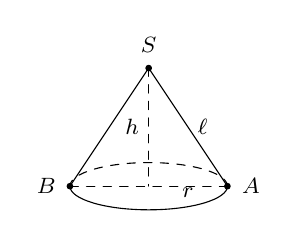
\begin{tikzpicture}[scale=1, font=\footnotesize, line join=round, line cap=round, >=stealth]
				\path
				(0,0) coordinate (O)
				(1,0) coordinate (A)
				(-1,0) coordinate (B)
				(0,1.5) coordinate (S)
				;
				\draw[dashed](A) arc (0:180:1cm and 0.3cm);
				\draw(A) arc (0:-180:1cm and 0.3cm);
				\draw (B)--(S)--node[right] {$\ell$}(A);
				\draw[dashed]  (B)--(O)--node[below,yshift=3pt] {$r$}(A) (S)--node[left] {$h$}(O);
				\foreach \d/\g in {S/90,B/180,A/0}{
					\draw[fill=black](\d) circle (1pt) +(\g:.3)node{$\d$};}
		\end{tikzpicture}}
	}
\end{ex}

\begin{ex}%[Đề TT, Sở Bà Rịa - Vũng Tàu, 2022 - 2023]%[Phạm Tiến Long , 12-EX-6-2023]%[2D2K6-3]
	Có bao nhiêu số nguyên $x$ thỏa mãn $\log _3 x+2 \log _x 9-5 \le 0$?
	\choice
	{\True $79$}
	{$80$}
	{$81$}
	{$27$}
	\loigiai{Điều kiện $x>0$ và $x\ne 1$.\\
		Ta có $\log _3 x+2 \log _x 9-5 \le 0
		\Leftrightarrow \log _3 x+4 \log _x 3-5 \le 0\Leftrightarrow \log _3 x+ \dfrac{4}{\log _3 x} -5 \le 0$.\\
		Đặt $t=\log _3 x$. Bất phương trình trên trở thành $t+\dfrac{4}{t}-5\le 0\Leftrightarrow \dfrac{t^2-5t+4}{t}\le 0$.\quad(1)\\
		Ta có $t^2-5t+4=0\Leftrightarrow \hoac{&t=1\\&t=4.}$\\
		Bảng xét dấu
		\begin{center}
			
\begin{tikzpicture}[scale=1, font=\footnotesize, >=stealth]
				\tikzset{t style/.style = {style = draw}}
				\tkzTabInit
				[lgt=2,espcl=2.5,deltacl=0.6,nocadre=false]
				{$t$/0.7,$t$/0.7,$t^2-5t+4$/0.7,$\dfrac{t^2-5t+4}{t}$/1}
				{$-\infty$,$0$,$1$,$4$,$+\infty$}
				\tkzTabLine{,-  , 0, +,t, + , t,+,}
				\tkzTabLine{,+  , t , +,0, - , 0,+,}
				\tkzTabLine{, -, d , +,0,-, 0,+,}
			\end{tikzpicture}
		\end{center}
		Dựa vào bảng xét dấu ta có $(1)\Leftrightarrow t<0$ hoặc $1\le t \le 4$.\\
		Với $t<0$ ta có $\log_3 x<0\Leftrightarrow x<1$.\\
		Với $1\le t \le 4$ ta có $1\le \log_3 x \le 4\Leftrightarrow 3 \le x \le 81$.\\
		Kết hợp với điều kiện ta có tập nghiệm của bất phương trình là $S=(0;1)\cup [3;81]$.\\
		Mà $m\in \mathbb{Z}$ nên $m\in \{3;4;\ldots;81\}$.\\
		Vậy có $79$ số nguyên $x$ thỏa mãn.
	}
\end{ex}

\begin{ex}%[Đề TT, Sở Bà Rịa - Vũng Tàu, 2022 - 2023]%[Phạm Tiến Long , 12-EX-6-2023]%[2D3K1-1]
	Cho hàm số $y=f(x)$ liên tục trên $\mathbb{R}$, có đồ thị $(C)$ và có đạo hàm cấp hai $f''(x)=6x+12$. Biết đồ thị $(C)$ đi qua điểm $M(-2;2)$ và tiếp tuyến của $(C)$ tại $M$ là đường thẳng $d\colon y=2x+6$. Khi đó giá trị của $f(3)$ bằng
	\choice
	{\True $137$}
	{$135$}
	{$131$}
	{$129$}
	\loigiai{
		\textbf{Cách 1.}\\
		Ta có $f'(x)=\displaystyle\int f''(x) \mathrm{\,d}x=\displaystyle\int (6x+12) \mathrm{\,d}x=3x^2+12x+C_1$.\\
		Mặt khác, hệ số góc tiếp tuyến là $f'(-2)=2$ nên $3(-2)^2+12(-2)+C_1=2 \Leftrightarrow C_1=14$.\\
	Suy ra	$ f'(x)=3x^2+12x+14 \Rightarrow f(x)=\displaystyle\int f'(x) \mathrm{\,d}x=\displaystyle\int (3x^2+12x+14) \mathrm{\,d}x=x^3+6x^2+14x+C_2$.\\
		Lại có $M(-2;2)\in (C) \Leftrightarrow (-2)^3+6(-2)^2+14(-2)+C_2=2 \Leftrightarrow C_2=14$.\\
		Vậy $f(x)=x^3+6x^2+14x+14$ và $f(3)=137$.\\
		\textbf{Cách 2.}\\	
		Vì hàm số $f$ có đạo hàm cấp hai là đa thức bậc nhất nên gọi $f(x)=ax^3+bx^2+cx+d$ (với $a,b,c,d \in \mathbb{R}$).\\
		Khi đó $f'(x)=3ax^2+2bx+c$ và $f''(x)=6ax+2b$.\\
		Theo giả thiết, ta có
		\begin{eqnarray*}
			& & \heva{& f''(x)=6x+12\\& M(-2;2)\in (C)\\& \text{hệ số góc tiếp tuyến là }f'(-2)=2}\Leftrightarrow \heva{& 6ax+2b=6x+12\\& a(-2)^3+b(-2)^2+c(-2)+d=2\\& 3a(-2)^2+2b(-2)+c=2}\\
			& \Leftrightarrow & \heva{& a=1,~b=6\\& -2c+d=-14\\& c=14}\Leftrightarrow \heva{& a=1,~ b=6\\& d=14\\& c=14.}
		\end{eqnarray*}
		Vậy $f(x)=x^3+6x^2+14x+14$ và $f(3)=137$.
	}
\end{ex}

\begin{ex}%[Đề TT, Sở Bà Rịa - Vũng Tàu, 2022 - 2023]%[Phạm Tiến Long , 12-EX-6-2023]%[2D1K2-2]
	\immini
	{
		Cho hàm số $y=f(x)=\dfrac{1}{4}x^4+a x^3+b x^2+c x$. Hàm số $y=f'(x)$ có đồ thị như hình vẽ bên. 
		Số điểm cực trị của hàm số $y=f\left(1-x^2\right)$ là
		\choice
		{$5$}
		{\True $3$}
		{$4$}
		{$2$}
	}
	{
		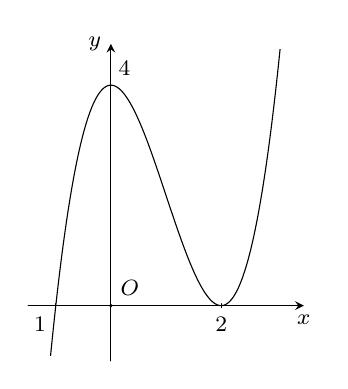
\begin{tikzpicture}[scale=0.7, font=\footnotesize, line join=round, line cap=round, >=stealth]
			\def\xmin{-1.5} \def\xmax{3.5}
			\def\ymin{-1} \def\ymax{4.75} 
			\draw[->] (\xmin,0)--(\xmax,0) node [below]{$x$};
			\draw[->] (0,\ymin)--(0,\ymax) node [left]{$y$};
			\clip (\xmin+0.1,\ymin+0.1) rectangle (\xmax-0.1,\ymax-0.1);
			\draw[smooth,samples=300] plot(\x,{((\x)+1)*((\x)-2)^2});
			\fill (0,0)circle (1pt)node[above right]{$O$};
			\foreach \x/\g in {-1/below left,2/below}  \draw[thin] (\x,1pt)--(\x,-1pt) node[\g]{$\x$};
			\foreach \y/\g in {4/above right} \draw[thin] (1pt,\y)--(-1pt,\y) node[\g]{$\y$};
		\end{tikzpicture}
	}
	\loigiai{
		Từ đồ thị ta có bảng xét dấu
		\begin{center}
			
\begin{tikzpicture}[scale=1, font=\footnotesize, line join=round, line cap=round, >=stealth]
				\tkzTabInit
				[lgt=1.2,espcl=2.5,deltacl=0.6,nocadre=false]
				{$x$/0.7,$f'(x)$/0.7}
				{$-\infty$,$-1$,$2$,$+\infty$}
				\tkzTabLine{, - , 0 , + ,0  , + ,}
			\end{tikzpicture}
		\end{center}
		Đặt $g(x)=f\left(1-x^2\right)$.\\
		Ta có $g'(x)=-2xf'\left(1-x^2\right)$.\\
		$g'(x)=0\Leftrightarrow \hoac{&x=0\\&1-x^2=-1\\&1-x^2=1}\Leftrightarrow \hoac{&x=1\\&x=\pm \sqrt{2}.}$\\
		Bảng xét dấu của $g'(x)$
		\begin{center}
			
\begin{tikzpicture}[scale=1, font=\footnotesize, line join=round, line cap=round, >=stealth]
				\tkzTabInit
				[lgt=1.2,espcl=2.5,deltacl=0.6,nocadre=false]
				{$x$/0.7,$g'(x)$/0.7}
				{$-\infty$,$-\sqrt{2}$,$0$,$\sqrt{2}$,$+\infty$}
				\tkzTabLine{, - , 0 , + ,0  ,- ,0,+}
			\end{tikzpicture}
		\end{center}
		Dựa vào bảng xét dấu ta thấy hàm số có $3$ điểm cực trị.
	}
\end{ex}

\begin{ex}%[Đề TT, Sở Bà Rịa - Vũng Tàu, 2022 - 2023]%[Phạm Tiến Long , 12-EX-6-2023]%[2D1K3-6]
	Anh Ba đang trên chiếc thuyền tại vị trí $A$ cách bờ sông $2$km, anh dự định chèo thuyền vào bờ và tiếp tục chạy bộ theo một đường thẳng để đến một địa điểm $B$ tọa lạc ven bờ sông, $B$ cách vị trí $O$ trên bờ gần với thuyền nhất là $4$km (hình vẽ). Biết rằng anh Ba chèo thuyền với vận tốc $6$ km/h và chạy bộ trên bờ với vận tốc $10$ km/h. Khoảng thời gian ngắn nhất để anh Ba từ vị trí xuất phát đến được điểm $B$ là
	\begin{center}
		\begin{tikzpicture}[font=\footnotesize, line join=round, line cap=round, >=stealth,scale=0.5,transform shape]
			%%Chiếc thuyền chèo
			\tikzset{Icon-thuyen/.pic={
					\fill[ball color=brown!80!cyan!80!white](-4.65,0.08)..controls+(-23:2.5) and+(-165:3.5)..(4.6,0)..controls+(15:0.15) and+(-15:0.5)..(3.9,0.2)..controls+(-172:5) and+(15:2)..(-4.65,0.08);
					%%Thành trong tầu
					\fill[ball color=gray!10!brown] [red](-4.65,0.08)--+(-25:0.4)..controls+(10:2) and++(-172:5)..(3.8,0)--++(110:0.2)..controls+(-172:5) and+(15:2)..(-4.65,0.08);
					
					\fill[ball color=gray!90!cyan](-4.65,0.08)..controls+(-23:2.5) and+(-165:3.5)..(4.6,0)..controls+(15:0.05) and++(65:1.2)..(4.2,-1)..controls++(-152:0.75) and+(13:2)..(-1,-2.5)..controls++(-167:1.1) and+(-50:3.5)..(-4.65,0.08);
					
					\fill[ball color=gray!90!cyan](2,0)coordinate(e)--++(0:0.4)--++(88:0.65)--++(175:0.3)coordinate(f)--cycle;
			}}
			%%Nhà trên bờ
			\tikzset{nha/.pic={
					\def\N{ 
						(-1.22,-.25)--(-.82,-.25)--(-.82,-.85)--(-1.22,-.85)--cycle;}
					\draw \N;
					\fill[brown] \N;
			}}
			\tikzset{cuaso/.pic={
					\def\C{ 
						(-1.22,-.25)--(-.82,-.25)--(-.82,-.85)--(-1.22,-.85)--cycle;}
					\draw \C;
					\fill[white] \C;
			}}
			\tikzset{cay/.pic={
					\def\C{ 
						(-1.25,-.85)--(-1.24,-.75)--(-1.22,-.75)--(-1.2,-.85)--cycle
						;}
					\def\L{ 
						(-1.23,-.78)
						..controls +(-40:.13) and +(-160:0.16) .. (-1.27,-.7)
						..controls +(-40:.13) and +(-160:0.14) .. (-1.23,-.6)
						..controls +(120:.0) and +(50:0.11) .. (-1.2,-.7)
						..controls +(60:.1) and +(0:0.2) .. (-1.23,-.78)
						--cycle
						;}
					
					\draw \C;
					\fill[black!50!white] \C;
					\draw \L;
					\fill[green] \L;
			}}
			%%Chim bay
			\tikzset{chim/.pic={
					\fill[blue](1.45,-1.25)..controls++(5:0.5)and++(180:0.75)..(3,-0.1)..controls++(0:0.5) and++(160:0.35)..(3.9,-0.8)..controls++(180:0.75) and++(-20:3.25)..(0,-3.32)..controls++(160:1) and++(5:0.5)..(-1.3,-3.1)..controls++(20:0.75) and++(180:0.75)..(1,-3.2)..controls++(0:2) and++(180:0.5)..(3.7,-0.75)..controls++(140:0.5) and++(0:0.25)..(3,-.35)..controls++(180:0.85)and++(-5:0.75)..(1.45,-1.25);
					\fill[blue](1.55,-1)..controls++(80:2.65) and++(-80:2.5)..(-1.5,4)..controls++(-88:2.5)and++(92:2.65)..(1.55,-1);
					\fill[blue](-1.5,4)..controls++(110:0.25) and++(108:1.5)..(-1.6,2.4)..controls++(140:1) and++(140:1)..(-1.25,0.8)..controls++(125:2) and++(140:1)..(-1.2,1.85)..controls++(115:1.5) and++(220:0.5)..(-1.5,4);
					\fill[blue](-1.6,0.9)..controls++(160:0.5) and++(138:1.2)..(-1.2,0)..controls++(-42:0.5) and++(140:1)..(-0.85,-1.8)..controls++(130:1) and++(-45:0.8)..(-1.1,0)..controls++(135:1) and++(190:0.05)..(-1.6,0.9);
					\fill[blue](-0.3,-1.9)..controls++(185:2) and++(-10:2)..(-3.9,-1.8)..controls++(-90:0.25) and++(160:0.5)..(-3.2,-2.4)..controls++(-140:0.5) and++(170:0.5)..(-2.8,-2.8)..controls++(-145:0.75) and++(-170:1)..(-2.1,-3.1)..controls++(-145:2)and++(-130:1)..(-1.8,-3.45)..controls++(-140:1)and++(-160:2)..(-1.5,-3)..controls++(-172:2.25)and++(-170:0.75)..(-2.05,-2.8)..controls++(178:1) and++(-178:2)..(-2.1,-2.45)..controls++(175:1.5) and++(-90:0.15)..(-3.7,-1.9)..controls++(-15:1.5) and++(195:1)..(-0.3,-1.9);
					\fill[blue,out=88,in=-160](2.1,-0.2)to(3.5,1.8)..controls++(-140:1) and++(80:0.5)..(2.1,-0.2);
					\fill[blue](1.2,1)..controls++(80:0.1) and++(180:0.1)..(1.8,1.3)..controls++(175:0.2) and++(90:0.25)..(1.2,1);
					\fill[blue](2,1.5)..controls++(40:0.25) and++(90:0.25)..(2.5,1.6)..controls++(90:0.25) and++(180:0.1)..(3.5,1.9)..controls++(160:0.2) and++(40:0.1)..(2.8,1.9)..controls++(90:0.25) and++(50:0.5)..(2,1.5);
			}}
			
			\begin{scope}%[opacity=0.75]
				\clip(-30,4)rectangle(5,-10);
				\fill[cyan!5](-30,10)rectangle(10,-10);
				\fill[orange!30!brown!30!white](-30,0)rectangle(10,-10);
				%%cù lao
				\fill [left color=brown!60!green,right color=brown!30!orange,line width=1.5pt,->,decorate,decoration={snake,amplitude=0.5mm,segment length=0.5 cm,post length=0.5 mm}](-10,0)..controls++(20:5) and++(-140:2)..(0,3)..controls++(-70:2) and++(170:3)..(10,0)--cycle;
				\foreach \x/\y [count=\i]in{-3/0.2,-5/0.7,5/0.2,3/0.4,0/1.2,-8/0,-2/2}
				\fill [cyan!30,decorate,decoration={snake,amplitude=0.5mm,segment length=1 cm,post length=0.5 mm}](-40,0.25)--++(60,0.25)--++(-90:1)..controls++(-140:15) and++(180:20)..(-40,-7)--cycle;
				
				\def\i{5}\def\j{-3}\def\s{6}		
				\path
				(-25,-0.5)pic[xscale=-0.5,yscale=0.5]{Icon-thuyen}%yslant=-0.25,
				(\i,\j)pic[scale=\s]{nha}
				(\i,\j)pic[fill=white,scale=.2*\s,,xshift=-4.7 cm,,yshift=-1.5 cm]{cuaso}
				(\i,\j)pic[fill=white,scale=.2*\s,,xshift=-4.1 cm,,yshift=-1.5 cm]{cuaso}
				(\i,\j)pic[fill=white,scale=.2*\s,,xshift=-3.5 cm,,yshift=-1.5 cm]{cuaso}
				(\i,\j)pic[fill=white,scale=.4*\s,,xshift=-1.55 cm,,yshift=-1.25 cm]{cuaso}
				(\i,\j)pic[scale=\s]{cay}
				(-5,3)pic[scale=0.15]{chim}
				;
				\draw(-25,-1)coordinate(A)--++(-45:10)coordinate(P)--++(0:16.7)coordinate(B)($(P)!(A)!(B)$)coordinate(O);
				\draw[dashed](A)--(O)node[pos=0.5,left]{$2$ km}--(P);
				\foreach \d/\g in{A/-160,B/-60,O/-135,P/-90}
				\draw[fill=black](\d)circle(1pt)node[shift={(\g:0.5)}]{$\d$};
				\draw[<->,dashed]([shift={(0,-1)}]O)--([shift={(0,-1)}]B)node[below,pos=0.5]{$4$ km};
			\end{scope}
		\end{tikzpicture}
	\end{center}
	\choice
	{\True  $40$ phút}
	{$44$ phút}
	{$30$ phút}
	{$38$ phút}
	\loigiai{
		Đặt $OP=x$ ($0<x<4$), suy ra $BP=4-x$ và $AP=\sqrt{4+x^2}$.\\
		Khoảng thời gian để anh Ba từ vị trí xuất phát đến vị trí $B$ là
		$$t=t_{AP}+t_{BP}=\dfrac{\sqrt{4+x^2}}{6}+\dfrac{4-x}{10}.$$
		Ta cần tìm $t_{\min}$. Ta có $t'(x)=\dfrac{x}{6\sqrt{4+x^2}}-\dfrac{1}{10}$ và $$t'(x)=0 \Leftrightarrow  \dfrac{x}{6\sqrt{4+x^2}}=\dfrac{1}{10}  \Leftrightarrow 3\sqrt{4+x^2} = 5x \Leftrightarrow \heva{& x \ge 0\\& 9(4+x^2)=25x^2} \Leftrightarrow x=\dfrac{3}{2} ~(\text{thỏa }0<x<4).$$
		Bảng biến thiên của hàm $t(x)$ như sau
		\begin{center}
			
\begin{tikzpicture}
				\tkzTabInit[nocadre=false, lgt=1.2, espcl=2.5, deltacl=0.6]
				{$x$/1,$t'(x)$/0.6,$t(x)$/2}
				{$0$, $\frac{3}{2}$, $4$}
				\tkzTabLine {,-,0,+,}
				\tkzTabVar{+/, -/$\frac{2}{3}$, +/}
			\end{tikzpicture}
		\end{center}
		Vậy khoảng thời gian ngắn nhất cần tìm là $t=\dfrac{2}{3}$ giờ, hay $t=40$ phút.
	}
\end{ex}

\begin{ex}%[Đề TT, Sở Bà Rịa - Vũng Tàu, 2022 - 2023]%[Phạm Tiến Long , 12-EX-6-2023]%[2H1G3-2]
	Cho hình chóp tam giác đều $S.ABC$ có cạnh đáy bằng $a$, khoảng cách giữa cạnh bên $SA$ và cạnh đáy $BC$ bằng $\dfrac{3a}{4}$. Thể tích khối chóp $S.ABC$ bằng
	\choice
	{$\dfrac{3a^3\sqrt{3}}{4}$}
	{$\dfrac{a^3\sqrt{3}}{4}$}
	{$\dfrac{a^3\sqrt{3}}{6}$}
	{\True $\dfrac{a^3\sqrt{3}}{12}$}
	\loigiai{
		\immini{
			Gọi $N$ là trung điểm của $BC$, $M$ là hình chiếu của $N$ trên $SA$, $H$ là hình chiếu của $S$ trên mặt phẳng $(ABC)$.\\
			Ta có $\heva{&BC \perp AN\\&BC\perp SH}\Rightarrow BC \perp (SAN)$.\\
			Mà $MN\subset (SAN) \Rightarrow BC\perp MN$.\\
			Suy ra $\mathrm{d}(SA,BC)=MN=\dfrac{3a}{4}$.\\
			Ta có $AM=\sqrt{AN^2-MN^2}=\sqrt{\left(\dfrac{a\sqrt{3}}{2}\right)^2+\left(\dfrac{3a}{4}\right)^2}=\dfrac{a\sqrt{3}}{4}$.
		}{
			\begin{tikzpicture}[scale=1, font=\footnotesize, line join=round, line cap=round, >=stealth]
				\def\a{0} \def\b{0} %tọa độ A
				\def\c{4} \def\d{0} %tọa độ B
				\def\e{1} \def\f{-1} %tọa độ C
				\pgfmathsetmacro\g{(\a+\c+\e)/3}%hoành độ G
				\pgfmathsetmacro\h{(\b+\d+\f)/3}%tung độ G
				\path
				(\a,\b) coordinate (A)
				(\c,\d) coordinate (C)
				(\e,\f) coordinate (B)
				(\g,\h) coordinate (H)
				(\g,3) coordinate (S)
				($(S)!0.6!(A)$) coordinate (M)
				($(B)!0.5!(C)$) coordinate (N)
				;
				\draw (S)--(A)--(B)--(S)--(C)--(B) (S)--(N);
				\draw[dashed] (A)--(C) (S)--(H) (A)--(N)--(M);
				\foreach \x/\g in {S/90,A/180,C/0,B/270,H/270,M/100,N/-20} \fill[black] (\x) circle (1pt)+(\g:0.3) node{$\x$};
		\end{tikzpicture}	}
\noindent 	Mặt khác ta có $\triangle AMN \backsim \triangle AHS$
$$\text{Suy ra } \dfrac{SH}{MN}=\dfrac{AH}{AM}\Rightarrow SH=\dfrac{MN\cdot AH}{AM}=\dfrac{MN\cdot \dfrac{2}{3}AN}{AM}=\dfrac{\dfrac{3a}{4}\cdot \dfrac{2}{3}\cdot \dfrac{a\sqrt{3}}{2}}{\dfrac{a\sqrt{3}}{4}}=a.$$
Thể tích khối chóp $S.ABC$ là $V=\dfrac{1}{3}SH\cdot S_{\triangle ABC}=\dfrac{1}{3}\cdot a \cdot \dfrac{a^2\sqrt{3}}{4}=\dfrac{a^3\sqrt{3}}{12}$.
	}
\end{ex}

\begin{ex}%[Đề TT, Sở Bà Rịa - Vũng Tàu, 2022 - 2023]%[Phạm Tiến Long , 12-EX-6-2023]%[2D3G3-3]
	Cho hàm số $y=f(x)$ không âm thỏa mãn điều kiện $f(x)f'(x)=2 x \sqrt{f^{2}(x)+1}$ và $f(0)=0$. Thể tích khối tròn xoay thu được khi quay hình phẳng giới hạn bởi các đường $y=f(x)$, $y=0$, $x=0$, $x=3$ quanh trục $Ox$ bằng
	\choice
	{$\dfrac{333}{5}$}
	{\True $\dfrac{333 \pi}{5}$}
	{$\dfrac{127089 \pi}{35}$}
	{$\dfrac{(11 \sqrt{11}-2 \sqrt{11}) \pi}{3}$}
	\loigiai{
		Ta có $f(x)f'(x)=2 x \sqrt{f^{2}(x)+1} \Leftrightarrow \dfrac{f(x)f'(x)}{\sqrt{f^{2}(x)+1}}=2x \Leftrightarrow \left(\sqrt{f^{2}(x)+1}\right)'=2x$.\\
		Lấy nguyên hàm $2$ vế ta được
		$\sqrt{f^{2}(x)+1}=\displaystyle\int (2x) \mathrm{\,d}x=x^2+C$.\\
		Thay $x=0$, ta được $\sqrt{f^{2}(0)+1}=0^2+C \Leftrightarrow C=1$ (do $f(0)=0$).\\
		Suy ra $\sqrt{f^{2}(x)+1}=x^2+1 \Rightarrow f^{2}(x)=(x^2+1)^2-1=x^4+2x^2$.\\
		Vậy thể tích khối tròn xoay thu được là 
		$$V=\pi \displaystyle\int f^2(x) \mathrm{\,d}x= \pi \displaystyle\int\limits_{0}^{3} \left(x^4+2x^2\right) \mathrm{\,d}x=\left(\dfrac{x^5}{5}+\dfrac{2x^3}{3}\right)\Big|_0^3=\dfrac{333 \pi}{5}.$$
	}
\end{ex}

\begin{ex}%[Đề TT, Sở Bà Rịa - Vũng Tàu, 2022 - 2023]%[Phạm Tiến Long , 12-EX-6-2023]%[2D3G2-3]
	Cho $
	\displaystyle\int\limits_0^{\tfrac{\pi}{3}} \dfrac{x\sin x}{2\cos^3 x}\mathrm{\,d}x=a\pi+b\sqrt{3}$ với $a$, $b$ là các số hữu tỉ. Giá trị của $a+b$ bằng
	\choice
	{\True $\dfrac{1}{12}$}
	{$\dfrac{7}{12}$}
	{$\dfrac{5}{6}$}
	{$-\dfrac{1}{6}$}
	\loigiai{
		Ta có $\displaystyle\int\limits_0^{\tfrac{\pi}{3}} \dfrac{x\sin x}{2\cos^3 x}\mathrm{\,d}x=\displaystyle\int\limits_0^{\tfrac{\pi}{3}} \dfrac{x\tan x}{2\cos^2 x}\mathrm{\,d}x$.\\
		Đặt $\heva{&u=\dfrac{x}{2}\\&\mathrm{d}v=\dfrac{\tan x}{2\cos^2 x}\mathrm{\,d}x=\tan x \mathrm{\,d}(\tan x)}\Rightarrow \heva{&\mathrm{d}u=\dfrac{1}{2}\mathrm{d}x\\&v=\dfrac{\tan^2 x}{x}.}$\\
		Suy ra
		\begin{eqnarray*}
			\displaystyle\int\limits_0^{\tfrac{\pi}{3}} \dfrac{x\sin x}{2\cos^3 x}\mathrm{\,d}x & =& \dfrac{x}{4} \tan^2 x\bigg|_0^{\tfrac{\pi}{3}}-\dfrac{1}{4}\displaystyle\int\limits_0^{\tfrac{\pi}{3}} \tan^2 x\mathrm{\,d}x\\
			&= & \dfrac{\pi}{4}-\dfrac{1}{4}\displaystyle\int\limits_0^{\tfrac{\pi}{3}} \left(\dfrac{1}{\cos^2 x}-1\right)\mathrm{\,d}x\\
			&= & \dfrac{\pi}{4}-\dfrac{1}{4}(\tan x-x)\bigg|_0^{\tfrac{\pi}{3}}=\dfrac{\pi}{3}-\dfrac{\sqrt{3}}{4}.
		\end{eqnarray*}
		Vậy $a=\dfrac{1}{3}$, $b=-\dfrac{1}{4}$. Vậy $a+b=\dfrac{1}{12}$.
	}
\end{ex}

\begin{ex}%[Đề TT, Sở Bà Rịa - Vũng Tàu, 2022 - 2023]%[Phạm Tiến Long , 12-EX-6-2023]%[2H3K3-7]
	Trong không gian $Oxyz$, gọi $(P)$ là mặt phẳng đi qua điểm $A(1;4;-3)$ và chứa trục $Ox$. Mặt cầu $(S)$ có tâm $I(1;2;1)$ và tiếp xúc với mặt phẳng $(P)$ có phương trình là
	\choice
	{\True $(x-1)^2+(y-2)^2+(z-1)^2=4$}
	{$(x+1)^2+(y+2)^2+(z+1)^2=4$}
	{$(x-1)^2+(y-2)^2+(z-1)^2=2$}
	{$(x+1)^2+(y+2)^2+(z+1)^2=2$}
	\loigiai{
		\immini{
			$(P)$ có cặp véc-tơ chỉ phương là $\overrightarrow{OA}=(1;4;-3)$ và $\overrightarrow{i}=(1;0;0)$ nên $(P)$ có $1$ véc-tơ pháp tuyến là $\overrightarrow{n}$ cùng phương với $\left[\overrightarrow{OA},\overrightarrow{i}\right]=(0;-3;-4)$, chọn $\overrightarrow{n}=(0;3;4)$.\\
			Mặt khác, $O(0;0;0)\in (P)$ nên $(P)$ có phương trình là $3y+4z=0$.\\
			Khi đó, $(S)$ có tâm $I(1;2;1)$ và bán kính $$R=\mathrm{d}\left(I,(P)\right)=\dfrac{|3\cdot2+4\cdot1|}{\sqrt{3^2+4^2}}=2.$$
			Vậy phương trình mặt cầu $(S)$ là $(x-1)^2+(y-2)^2+(z-1)^2=4$.
		}{
			\begin{tikzpicture}[scale=0.7,>=stealth, font=\footnotesize, line join=round, line cap=round]
				\clip (-4,-4.7) rectangle (4,2.3);
				\def \x{2}  \def \y{0.8} %bán kính trục lớn và trục bé elip
				\path
				(0,0) coordinate (I) 
				(-\x,0) coordinate (A) 
				(\x,0) coordinate (B)
				(-90:\x) coordinate (H)
				($(H)+(-\x-2,-\y)$) coordinate (m)
				($(H)+(\x+1,-\y)$) coordinate (n)
				($(H)+(\x+2,\y)$) coordinate (p)
				($(m)+(p)-(n)$) coordinate (q)
				($(H)+(\x,0.25)$) coordinate (O)
				($(O)+(-150:1.5)$) coordinate (x)
				;
				\tkzDrawCircle[radius](I,A)
				\draw[dashed] (A)--(B) arc (0:180:\x cm and \y cm);
				\draw (B) arc (0:-180:\x cm and \y cm);
				\tkzInterLC(p,q)(I,A)\tkzGetPoints{p'}{q'}
				\draw[dashed] (p')--(q') (I)--(H);
				\draw (q')--(q)--(m)--(n)--(p)--(p');
				\draw[->] (O)--(x);
				\foreach \d/\g in {I/90,H/-90,O/90,x/0}{
					\draw[fill=black](\d) circle (1pt) +(\g:.3)node{$\d$};}
				\tkzMarkAngles[size=0.7cm,arc=l](n,m,q)
				\tkzLabelAngles[pos=0.38](n,m,q){$P$}
				\node at (-1,0)[above]{$R$};
				\node at (-1.5,1.4)[above]{$(S)$};
				\draw[fill=black]($(O)+(-20:1)$) circle (1pt) +(0:.3)node{$A$};
		\end{tikzpicture}	}
	}
\end{ex}

\begin{ex}%[Đề TT, Sở Bà Rịa - Vũng Tàu, 2022 - 2023]%[Phạm Tiến Long , 12-EX-6-2023]%[2D2K5-5]
	Có bao nhiêu cặp số nguyên $(x;y)$ thỏa mãn $0\le x \le 2023$ và $\log_2 (2x+2)+x=2y+4^y$?
	\choice
	{$2022$}
	{\True $6$}
	{$2023$}
	{$4$}
	\loigiai{
		Ta có $\log_2 (2x+2)+x=2y+4^y\Leftrightarrow \log_2 (x+1)+x+1=2y+2^{2y}$.\\
		Xét hàm số $f(t)=t+2^t$.\\
		Ta có $f'(t)=1+2^t\ln2>0\Rightarrow $ $f(t)$ đồng biến trên $\mathbb{R}$.\\
		Suy ra $\log_2 (x+1)=2y\Leftrightarrow x+1=2^{2y}\Leftrightarrow x=4^y-1$.\\
		Ta có $0\le x \le 2023\Leftrightarrow 0\le 4^y-1 \le 2023\Leftrightarrow 1 \le 4^y \le 2024 \Leftrightarrow 0\le y\le \log_4{2024}\approx 5{,}49$.\\
		Mà $y\in\mathbb{Z}$ nên $y\in \{0;1;2;3;4;5\}$.\\
		Với mỗi giá trị $y$ thì có duy nhất $1$ giá trị $x$ thỏa mãn.\\
		Vậy có $6$ cặp số nguyên $(x;y)$ thỏa mãn yêu cầu bài toán.
	}
\end{ex}

\begin{ex}%[Đề TT, Sở Bà Rịa - Vũng Tàu, 2022 - 2023]%[Phạm Tiến Long , 12-EX-6-2023]%[2H2K1-2]
	Cho hình nón đỉnh $S$, đường cao $SO$. Gọi $A$ và $B$ là hai điểm thuộc đường tròn đáy hình nón sao cho khoảng cách từ $O$ đến $AB$ bằng $a$ và $\widehat{SAO}=30^{\circ}$, $\widehat{SAB}=60^{\circ}$. Diện tích xung quanh hình nón bằng
	\choice
	{$\pi a^2\sqrt{6}$}
	{$2 \pi a^2\sqrt{3}$}
	{\True $\pi a^2\sqrt{3}$}
	{$\dfrac{\pi a^2\sqrt{6}}{2}$}
	\loigiai{
		\immini{
			Gọi $r$, $h$, $\ell$ lần lượt là bán kính đáy, chiều cao, đường sinh của hình nón.\\
			Gọi $H$ là trung điểm của $AB$. Khi đó $OH=\mathrm{d}\left(O, AB\right)=a$.\\
			Xét $\triangle SOA$ vuông tại $O$, có $SA=\dfrac{SO}{\sin 30^{\circ}}=2h$.\\
			Vì $\triangle SAB$ cân tại $S$ có $\widehat{SAB}=60^{\circ}$ nên $\triangle SAB$ là tam giác đều, suy ra $SH=SA\cdot \dfrac{\sqrt{3}}{2}=h\sqrt{3}$.
		}{
			\begin{tikzpicture}[scale=0.8, font=\footnotesize, line join=round, line cap=round, >=stealth]
				\path
				(0,0) coordinate (O)
				(2,0) coordinate (B)
				(-2,0) coordinate (B')
				(0,3) coordinate (S)
				(-80:2cm and 0.6cm) coordinate (A)
				($(A)!.5!(B)$) coordinate (H)
				;
				\draw[dashed](B) arc (0:180:2cm and 0.6cm);
				\draw(B) arc (0:-180:2cm and 0.6cm);
				\draw (B')--(S)--node[right] {$\ell$}(B) (S)--(A);
				\draw[dashed]  (A)--(B)--(O)--node[left,yshift=3pt] {$r$}(A) (S)--node[left] {$h$}(O)--(H)--(S);
				\foreach \d/\g in {S/90,B/0,A/-90,O/135,H/0}{
					\draw[fill=black](\d) circle (1pt) +(\g:.3)node{$\d$};}
		\end{tikzpicture}	}
		\vspace*{-0.5cm}	\noindent
		Xét $\triangle SOH$ vuông tại $O$, có $SH^2=SO^2+OH^2\Leftrightarrow 3h^2=h^2+a^2\Rightarrow h=\dfrac{a\sqrt{2}}{2}$.\\
		Do đó $r=\dfrac{SO}{\tan 30^{\circ}}=h\sqrt{3}=\dfrac{a\sqrt{6}}{2}$ và $\ell = SA=a\sqrt{2}$.\\
		Vậy diện tích xung quanh cần tìm là $S_{\text{xq}}=\pi r \ell =\pi\cdot \dfrac{a\sqrt{6}}{2}\cdot a\sqrt{2}=\pi a^2\sqrt{3}$.
	}
\end{ex}

\begin{ex}%[Đề TT, Sở Bà Rịa - Vũng Tàu, 2022 - 2023]%[Phạm Tiến Long , 12-EX-6-2023]%[2H3G1-4]
	Trong không gian $Oxyz$, cho  ba điểm $A(1;4;5)$, $B(3;4;0)$, $C(2;-1;0)$ và mặt cầu $(S)\colon (x-1)^2+(y+1)^2+(z-3)^2=4$, điểm $N$ thay đổi trên mặt cầu $(S)$. Gọi $M$, $m$ lần lượt là giá trị lớn nhất và giá trị nhỏ nhất của biểu thức $P=NA^2+NB^2+3NC^2$. Giá trị $M-m$ bằng
	\choice
	{$125$}
	{\True $120$}
	{$80$}
	{$85$}
	\loigiai{
		Mặt cầu $(S)$ có tâm $E(1;-1;3)$ và bán kính $R=2$.\\
		Ta có
		\begin{eqnarray*}
			P &= & NA^2+NB^2+3NC^2\\
			&= & \left(\overrightarrow{NI}+\overrightarrow{IA}\right)^2+\left(\overrightarrow{NI}+\overrightarrow{IB}\right)^2+3\left(\overrightarrow{NI}+\overrightarrow{IC}\right)^2\\
			&= & 5\overrightarrow{NI}^2+2\overrightarrow{NI}\left(\overrightarrow{IA}+\overrightarrow{IB}+3\overrightarrow{IC}\right)^2+\overrightarrow{IA}^2+\overrightarrow{IB}^2+3\overrightarrow{IC}^2.
		\end{eqnarray*}
		Ta cần điểm $I$ thỏa $\overrightarrow{IA}+\overrightarrow{IB}+3\overrightarrow{IC}=\overrightarrow{0}\Rightarrow I(2;1;1)$.\\
		Khi đó $P=5\overrightarrow{NI}^2+\overrightarrow{IA}^2+\overrightarrow{IB}^2+3\overrightarrow{IC}^2=5NI^2+IA^2+IB^2+3IC^2$.\\
		Do $I$, $A$, $B$, $C$ là các điểm cố định nên $M-m=5NI_{\max}^2-5NI_{\min}^2=5(IE+R)^2-5(IE-R)^2=120$.
	}
\end{ex}

\begin{ex}%[Đề TT, Sở Bà Rịa - Vũng Tàu, 2022 - 2023]%[Phạm Tiến Long , 12-EX-6-2023]%[2D1G1-4]
	Cho hàm số $y=f(x)$ liên tục trên $\mathbb{R}$. Biết rằng $f'(2023)=0$ và $f''(x)<0, \forall x \in \mathbb{R}$. Xét hàm số $h(x)=f\left(\cot ^2 x-2\cot x+2024\right)$ trên khoảng $(0;\pi)$. Khẳng định nào dưới đây là đúng?
	\choice
	{\True $h(1)-h(2)>0$}
	{$h(2)-h(3)<0$}
	{$h\left(\dfrac{\pi}{2}\right)-h\left(\dfrac{\pi}{4}\right)>0$}
	{$h\left(\dfrac{\pi}{6}\right)-h\left(\dfrac{\pi}{4}\right)>0$}
	\loigiai{
		Vì $f''(x)<0, \forall x \in \mathbb{R}$ nên $f'(x)$ nghịch biến trên $\mathbb{R}$.\\
		Mà $f'(2023)=0$ nên $x=2023$ là nghiệm duy nhất của phương trình $f'(x)=0$.\\
		Ta có $h'(x)=-\dfrac{2}{\sin ^2 x}(\cot  x-1)\cdot f'\left(\cot ^2 x-2\cot x+2024\right)$ và $$h'(x)=0\Leftrightarrow \hoac{& \cot  x=1\\& \cot ^2 x-2\cot x+2024=2023} \Leftrightarrow \cot x=1 \Leftrightarrow x=\dfrac{\pi}{4}+k\pi,~(k\in \mathbb{Z}).$$
		Xét trên $(0;\pi)$, bảng biến thiên của $h(x)$ như sau
		\begin{center}
			
\begin{tikzpicture}
				\tkzTabInit[nocadre=false, lgt=1.2, espcl=2.5, deltacl=0.6]
				{$x$/0.7,$y'$/0.6,$y$/2}
				{$0$, $\frac{\pi}{4}$, $\pi$}
				\tkzTabLine {,+,0,-,}
				\tkzTabVar{-/, +/$h\left(\frac{\pi}{4}\right)$, -/}
			\end{tikzpicture}
		\end{center}
		Dựa vào bảng biến thiên, ta thấy $h(x)$ nghịch biến trên $\left(\dfrac{\pi}{4};\pi\right)$ nên $h(1)>h(2) \Leftrightarrow h(1)-h(2)>0$. 
	}
\end{ex}

\Closesolutionfile{ans}
\begin{indapan}{10}
	{ans/ans-2-TT-22-SGD-BaRiaVungTau-23}
\end{indapan}

